\documentclass[a4paper]{article}

\usepackage[utf8]{inputenc}
\usepackage[serbian]{babel}
\usepackage{listings}
\usepackage{caption}
\usepackage{url}
\usepackage{amsmath}
\usepackage{amssymb}
\usepackage[]{algorithm2e}
\usepackage{graphicx}
\usepackage{xcolor,colortbl}
\usepackage[unicode]{hyperref}
\hypersetup{colorlinks,citecolor=green,filecolor=green,linkcolor=blue,urlcolor=blue}

\definecolor{Gray}{gray}{0.82}

\graphicspath{{./img/}}

\title{Optimizacija maksimalne k-zadovoljivosti\\ populacionim metahauristikama\\ \small{Seminarski rad u okviru kursa\\ Računarska inteligencija\\ Matematički fakultet, Beograd}}

\author{David Dimić, Zorana Gajić \\ daviddimic@hotmail.com, zokaaa\_gajich@bk.ru}
\date{Maj 2019.}

% text width and height
\textwidth 14cm
\textheight 22cm

% distance from the top
\voffset -1.5cm

% distance from the left
\hoffset 0.5cm
\oddsidemargin 0mm

% distance from the bottom
\footskip 1.5cm

\begin{document}

\maketitle


\abstract{
U ovom radu biće objedinjene, implementirane i upoređene dve grupe algoritama za rešavanje
optimizacionog problema maksimalne k-zadovoljivosti zasnovane na populacijama - 
evolucioni algoritmi razvijeni u nekoliko različitih varijanti SAWEA, RFEA, FlipGA
i ASAP, i rojevi čestica PSO sa verzijama PSO-LS, PSOSAT i WPSOSAT. Biće iznete njihove
osobine, prednosti, mane i unapređenja, da bi se na kraju, na konkretnim rezultatima 
implementiranih algoritama pokazale njihove razlike i mogućnosti.}

\setcounter{tocdepth}{2} 
\tableofcontents

\newpage


\section{Uvod}
\label{sec:uvod}
Na početku, potrebno je jasno formulisati problem da bi se pristupilo njegovom rešavanju.
Problem maksimalne k-zadovoljivosti može se definisati na sledeći način: 
Neka je data je formula $F$ u KNF obliku sa $n$ 
promenjivih $(x_1, x_2, ..., x_n)$ i $m$ klauza.
Klauza $C_i$ dužine $k$ je disjunkcija $k$ literala: 
$C_i = (x_1  \vee x_2 ... \vee x_k)$, gde je svaki literal promenljiva ili 
njegova negacija i može se pojavljivati više puta u izrazu.
Cilj je pronaći istinitosne vrednosti promenljivih, valuaciju koja je 
vektor $\vec{v} = (x_1, x_2, ..., x_n) \in \{ 0,1 \}^n$ tako da ova valuacija 
maksimizuje broj zadovoljenih klauza u formuli $F$.\\

Ako valuacija zadovoljava formulu, onda se ona naziva modelom formule $F$. 
Max k-SAT problem može se definisati parom $(\Omega, SC)$, gde je $\Omega$ skup svih
potencijalnih rešenja iz $\{0,1\}^n$, vektor $n$ promenljivih, 
a $SC:\Omega \rightarrow \mathbb{N}$, skor valuacije koji je jednak broju zadovoljenih klauza. 
Shodno ovome, problem max k-SAT je naći $\vec{v} \in \Omega$ za koje je $SC$ maksimalno:
$$\max_{\vec{v} \in \Omega}\{SC(\vec{v})\}$$

Očigledno, ima $2^n$ potencijalnih rešenja koji zadovoljavaju formulu $F$. 
Dokazano je da je problem max k-SAT je NP-kompletan za svako $k>2$ \cite{NP-complete}.\\

%Pregled poglavlja
Kroz dalja poglavlja pristupiće se rešavanju ovako formulisanog problema prvo evolucionim
algoritmima (EA) \ref{sec:ea}, gde će biti reči o osnovnim osobinama, 
biće dat njegov pseudokod i objašnjenja svake od akcija koje se preduzimaju. 
Potom će biti iznete nekoliko verzija  algoritma
\footnote{Sve implementacije dostupne su na GitHub nalogu autora: \\
\url{https://github.com/zokaaagajich/max-k-sat}} 
i njihova unapređenja u delu \ref{sec:ea_varijante} i prikazane njihove mogućnosti
u rezultatima \ref{sec:ea_rezultati}. U drugom delu biće predstavljena optimizacija
rojem čestica (PSO) \ref{sec:pso} u njegovoj diskretnoj formi sa nekoliko različitih verzija
\ref{sec:pso_varijante} koji će biti upoređeni u rezultatima \ref{sec:pso_rezultati}.


\section{Evolucioni algoritmi (EA)}
\label{sec:ea}
Evolucioni algoritmi \cite{vi_Janicic} bazirani su na Darvinovoj teoriji evolucije, 
u kojoj unutar jedne populacije najčešće opstaju najbolje prilagođene jedinke. 
Reprezentacija jedinke naziva se hromozom ili genotip. 
Cilj je naći vrednost za koju zadata funkcija cilja dostiže svoj ekstremum 
ili vrednost koja je dovoljno blizu ekstremuma. Hromozomi su obično predstavljeni
nizovima nula i jedinica, ali moguće su i druge reprezentacije. 
Postupak se odvija kroz generacije.\\

Tokom izvršavanja algoritma u svakoj generaciji postoji isti broj jedinki i za svaku od
njih izračunava se njihov kvalitet, odnosno funkcija prilagođenosti.
Ova funkcija naziva se i fitnes funkcija.
Iz jedne generacije se na osnovu vrednosti fitnes funkcije, 
kroz proces selekcije biraju jedinke koje će biti iskorišćene za stvaranje novih jedinki. 
One kvalitetnije se biraju sa većom verovatnoćom. 
Videćemo različite tehnike selekcija kao što su turnirska i ruletska. \\

Nad izabranim jedinkama primenjuju se genetski operatori ukrštanja
i tako se dobijaju nove jedinke. Ukrštanjem se od dve jedinke dobija nova (ili dve nove) sa
genetskim materijalom koji je dobijen neposredno od roditelja, 
tj. od polaznih jedinki. U ovom radu korišćeno je samo uniformno ukrštanje. \\

Operatorom mutacije može da se modifikuje deo polazne jedinke i dobije nov genetski materijal. 
U svakoj generaciji može da dođe do rekombinacije gena zbog koje se 
javlja sličnost ali i različitost između jedinki iste generacije. 
Biće izložene različite vrste mutacija: slučajna, zasnovana na znanju, jednog bita i ostale. \\

Politika zamene generacija određuje kako se od postojećih jedinki i 
njihovog potomstva kreira nova generacija. Neke jedinke u novoj generaciji mogu biti bolje,
a neke lošije od jedinki u prethodnoj generaciji. \\

Kriterijumi zaustavljanja mogu biti razni. U ovom radu korišćeno je zaustavljanje 
kada se dostigne maksimalan broj unapred zadatih iteracija, ili kada sve klauze 
formule $F$ postanu zadovoljene. 
Tada je formula u potpunosti zadovoljena pa nema potrebe za daljom pretragom.\\

Naredni pseudok\^ od \ref{alg:EA} sumira objašnjene faze osnovnog EA na kojem se dalje
zasnivaju ostale varijante. U narednim poglavljima biće opisan 
svaki od pojedinačnih delova koji čini ovaj algoritam, a koji će se nadalje koristiti: 
fitnes funkcija, selekcija, ukrštanje i mutacija, kao i neke od njihovih adaptacija.\\

\begin{algorithm}[H]
\SetAlgoLined
\SetKwInOut{Input}{Input}
\SetKwInOut{Output}{Output}

\Input{Formula $F$ u KNF-u, $n$ i $m$}
\Output{Najbolja procenjena valuacija i broj zadovoljenih klauza}
\BlankLine
 inicijalizacija populacije\;
 t = 0; \tcp*[h]{tekuća iteracija}\\
 \While{nije zadovoljen uslov zaustavljanja}{
  t = t + 1\;
  Određivanje funkcije prilagođenosti svake jedinke\;
  Selekcija jedinki za primenu genetskih operatora\;
  Ukrštanje za izabrane parove jedinki\;
  Mutacija izabranih jedinki\;
 }
\caption{Osnovni evolutivni algoritam}\label{alg:EA}
\end{algorithm}


\subsection{Inicijalizacija rešenja}
\label{sec:ea_init}
Populaciju jedinki jedne generacije čini skup hromozoma, odnosno rešenja problema.
Hromozome možemo predstaviti na različite načine, ali će ovde biti korišćeno
prirodno predstavljanje nizom binarnih cifara.
Potrebno je da inicijalizujemo hromozome pseudoslučajnim brojevima \{0, 1\}.
Veoma važnu ulogu igra odabir parametara. Parametri mogu biti fiksni ili im se vrednosti 
mogu na određen način menjati iz generacije u generaciju.


\subsection{Fitnes funkcija}
\label{sec:ea_fitness}
U različitim verzijama EA koriste se različite funkcije prilagođenosti, koja je od suštinske
važnosti za dobro rešavanje problema. 
Prva fitness funkcija koja se sama nameće jeste broj zadovoljenih klauza, 
koja će biti upotrebljena u FlipGA i ASAP algoritmima.

	\begin{center}
	$ f_{MAXSAT} (x) = \sum_{k=1}^{N} f(x, c_k) $
	\end{center} 
	
gde je $N$ ukupan broj klauza, $x$ predstavlja jedan hromozom $i$

	\begin{center}
$ f(x, c_k) = \begin{cases} 1, & \mbox{ako je klauza } c_k \mbox{ zadovoljena hromozomom } x \\ 0, & \mbox{inače.} \end{cases} $
	\end{center}
Nešto komplikovanije funkcije prilagođenosti su SAW i REF koje se koriste
u SAWEA i RFEA algoritmima.


\subsubsection{SAW}
\label{sec:fitness_saw}
Eiben i van der Hauw su razvili evolutivni algoritam koji koristi stepenasto prilagođavanje
težina (eng.~{\em stepwise adaptation of weights}). Svakoj klauzi $c_i$ pridružuje se težina 
$w_i$, u početku inicijalizovana sa jedan. Ove težine se potom, posle određenog vremena,
ažuriraju po pravilu:  

	\begin{center}
	$ w_i = w_i + \Delta w $
	\end{center}
gde je $\Delta w$:
	\begin{center}
	$ \Delta w = 1 - f(x^*, c_i) $
	\end{center}
gde $f$ označava da li je klauza $c_i$ zadovoljena trenutno najboljim
hromozomom $x^*$. Stoga, $\Delta w$ može biti samo 1, ako $c_i$ nije zadovoljena, 
ili 0, ako jeste. Iz ovoga se vidi da se težine nezadovoljenih klauza vremenom uvećavaju
i time se pretraga usmerava ka njima. \\

Finalno za jedan hromozom $ i $ definišemo funkciju prilagođenosti kao:

	\begin{center}
	$ f_{SAW}(i) = w_1 f(i, c_1) + ... + w_N f(i, c_N) = \sum_{k=1}^{N} w_k f(i, c_k)	$
	\end{center}


\subsubsection{REF}
\label{sec:fitness_rfea}
Gotlieb i Vos \cite{GotVos98_f_ref} predstavili su koncept funkcija prerada 
(eng.~{\em refining functions}) koje su nastale iz želje da se prevaziđe mana obične 
funckije prilagođenosti koja često vraća isti rezultat za različite hromozome. 
Definišemo je koristeci $f_{MAXSAT}$ za hromozom $x$ na sledeći način:

\begin{center}
	$ f_{REF} (x) = f_{MAXSAT} (x) + \alpha r(x) $
\end{center}
gde je $\alpha > 0 $ predstavlja nivo uticanja funkcije $r$, 
$ r : \lbrace 0, 1 \rbrace ^ n \rightarrow [0, 1 \rbrace $. 
Za $\alpha = 0 $ $f_{REF} $ se ponaša kao $f_{MAXSAT} $. \\

Funkcija $r$ za hromozom $x$ se definiše na sledeći način:

\begin{center}
$r(x) = \dfrac{1}{2} ( 1 + \dfrac{\sum_{i=1}^{N} K(x_i) v_i} {1+ \sum_{i=1}^{N} |v_i|})$
\end{center}
gde  $ K(0) = -1, K(1) = 1 $. Autori su predložili da ažuriranje $v_i$  izgleda ovako:
 
\begin{center}
	$ v_i = v_i - K(x^*) \sum_{k \in U_i(x^*)} w_k $
\end{center}
gde je $x^*$ trenutno najbolja jedinka, $U_i (x^*)$ je skup nezadovoljenih klauza 
u kojima se pojavljuje promenljiva $i$, $w_k$ je definisano na isti način kao i u
\ref{sec:fitness_saw}. $v_i$ predstavlja težine promenljivih. Visoke pozitivne težine 
ukazuju da se za odgovarajuće promenljive preferira da budu 1, dok za negativne 0. 
Inicijalno, sve težine promenljivih su postavljene na vrednost 0.


\subsection{Selekcija}
\label{sec:ea_selekcija}
Selekcija predstavlja izbor jedinki iz trenutne populacije koje će biti korišćene za dobijanje
naredne generacije. Ona obezbeđuje čuvanje i prenošenje dobrih osobina populacije. 
U ovom radu koriste se dve najpopularnije strategije selekcije: ruletska i turnirska.

\subsubsection{Ruletska selekcija}
\label{sec:ea_ruletska}
Ruletska selekcija (eng.~{\em roulette wheel selection}) \cite{vi_Janicic} je proces 
selekcije u kojem veće šanse da učestvuju u reprodukciji imaju prilagođenije jedinke.
Ako $f(i)$ vrednost funkcije prilagođenosti za jedinku $i$ , a $N$ broj jedinki u populaciji,
verovatnoća da će jedinka $i$ biti izabrana da učestvuje u reprodukciji je:

\begin{center}
$p_i = \dfrac{f(i)}{\sum_{j}^{N} f(j)} $
\end{center}
Ovako definisana ruletska selekcija imaće primenu u FlipGA algoritmu.

\subsubsection{Turnirska selekcija}
\label{sec:ea_turnirska}
U turnirskoj selekciji \cite{vi_Janicic} jedinke odigravaju turnire u kojima veće šansu za
pobedu imaju one sa boljom prilagođenošću. Za jedan turnir bira se slučajno $k$ jedinki iz
populacije. Pobednikom se smatra jedinka sa najvećom prilagođenošću. 
Turnirska selekcija primnjuje se u RFEA.

\subsection{Ukrštanje}
 \label{sec:ea_ukrstanje}
Ukrštanje \cite{vi_Janicic} je proces u kome učestvuju dve jedinke koje se nazivaju roditelji. 
Rezultat ukrštanja je jedna nova jedinka ili dve nove jedinke koje nazivamo decom, koje
za cilj imaju kombinovanje gena oba roditelja radi postizanja boljih osobina.
U FlipGA algoritmu biće korišćeno uniformno ukrštanje.
Uniformno ukrštanje daje dva deteta. Kod ovog ukrštanja svaki bit prvog roditelja 
se sa verovatnoćom $p$ prenosi na prvo dete, a sa verovatnoćom $1-p$ na drugo dete. 
Za verovatnoću $p$ uzeta je vrednost 0.5. 

\begin{table}[h!]
\centering
\captionof{table}{Uniformno ukrštanje}\label{tab:ea_ukrstanje} 
\begin{tabular}{|*{6}{c|}}
  \multicolumn{6}{c}{Dva roditelja} \\ \hline
  \rowcolor{Gray}  
  1 & 0 & 0 & 0 & 1 & 1 \\ \hline
  0 & 0 & 1 & 1 & 0 & 1 \\ \hline
  \multicolumn{6}{c}{Dva deteta} \\ \hline
  \cellcolor{Gray} 1 & 0 & 1 & \cellcolor{Gray} 0 & 0 & \cellcolor{Gray} 1 \\ \hline
  0 & \cellcolor{Gray} 0 & \cellcolor{Gray} 0 & 1 & \cellcolor{Gray} 1 & 1 \\ \hline
\end{tabular}
\end{table}


\subsection{Mutacija}
 \label{sec:ea_mutacija}
Mutacija \cite{vi_Janicic} se primenjuje nakon operatora ukrštanja 
(ako se on uopšte i primenjuje). 
To je operator koji sa određenom verovatnoćom menja jedan deo jedinke na određeni način. 
Uloga mutacije je da spreči da jedinke u populaciji postanu suviše slične 
i da pomogne u obnavljanju izgubljenog genetskog materijala.
U narednom delu biće izložene neke od mutacija koje će se koristiti u 
različitim varijantama EA algoritama, koji će biti objašnjeni u poglavlju
\ref{sec:ea_varijante}.

\subsubsection{Slučajna mutacija}
\label{sec:ea_slucajna_mutacija}
Slučajna mutacija (eng.~{\em random mutation}) primenjuje se nad celim hromozomom 
tako što za svaki gen na slučajan način bira vrednost $t \in [0,1]$ 
i ako je ta vrednost manja od zadatog parametra mutiranja $mutation\_rate$ 
tj. $ t < mutation\_rate$ onda se vrši invertovanje tog gena.
Ovakav operator mutiranja biće korišćen u FlipGA algoritmu \ref{sec:ea_flipga}.

\subsubsection{Mutacija jednog bita}
\label{sec:ea_mutacija_one}
Za razliku od slučajne mutacije koja je prolazila kroz ceo hromozom i menjala gene u
zavisnosti od slučajnog broja, u mutaciji jednog bita (eng.~{\em mutation one operator})
bira se proizvoljno tačno jedan gen koji se potom menja. 
Ova mutacija koristiće se u SAWEA verziji \ref{sec:ea_sawea}.

\subsubsection{Slučajno-prilagodljiva mutacija}
\label{sec:ea_slucajno_prilagodljiva_mutacija}
Slučajno-prilagodljiva mutacija (eng.~{\em random-adaptive mutation}) \cite{adaptiveEA} 
je u svojoj srži zapravo slučajna mutacija sa jednom izmenom:
Neki geni hromozoma mogu biti ,,zamrznuti'' radi očuvanja dobrog rešenja do kog se došlo,
dok se ostali, za koje se utvrdilo da ne vode do rešenja, mogu menjati.\\

Ova ideja uvodi se u ASAP algoritmu \ref{sec:ea_asap} gde će biti detaljnije obrađena.
Dakle, ova mutacija radi isto kao slučajna mutacija, osim kada naiđe na ,,zamrznuti'' gen.
U tom slučaju ne radi ništa i prelazi na sledeći gen hromozoma.

\subsubsection{Mutacija zasnovana na znanju}
\label{sec:ea_mutacija_znanje}
Kod mutacije zasnovane na znanju (eng.~{\em knowledge-based mutation}) \cite{ea_with_table}
pokušavamo da iskoristimo nešto što znamo o trenutnom rešenju
i da ne vršimo mutaciju na potpuno slučajan način.
Mutaciju ćemo vršiti nad onim hromozomima koje nismo zadovoljili, 
jer će možda, posle mutacija nad njima, postati zadovoljene i time uvećati broj ukupno
zadovoljenih klauza.\\

Za dati hromozom, koji predstavlja
tekuće rešenje, možemo naći skup nezadovoljenih klauza. 
Iz skupa nezadovoljenih klauza na slučajan način biramo tačno jednu klauzu, 
a potom iz nje, ponovo, biramo jednu njenu promenljivu koju ćemu mutirati. 
Primena ove mutacije nalazi se u RFEA algoritmu \ref{sec:ea_rfea}.

\subsubsection{Lamarckian SEA-SAW mutacija}
\label{sec:ea_lamarckian}
Da bi se poboljšali SAWEA i RFEA algoritmi koristi se Lamarckian mutacija koju su predstavili 
de Jong i Kosters \cite{ea_without_table, ea_with_table}. 
Ovakav operator mutacije liči na lokalnu pretragu, naime, 
nakon dobijanja dece za novu populaciju bira se jedno dete $c$ na slučajan način.
Takođe, kreiramo skup slučajno odabranih klauza. 
Ako je svaka klauza u ovakvom skupu zadovoljena hromozomom $c$ onda se ne radi ništa. 
Inače, izabere se jedna slučajna promenljiva u nezadovoljenoj klauzi i mutira se.


\subsection{Politika zamene generacija}
\label{sec:ea_zamena}
Jedna od podgrupa EA su evolucione strategije ES (eng.~{\em Evolution Strategy}) koje
koriste selekciju, mutaciju i neku od politika zamene.
Politika zamene generacije \cite{vi_Janicic, ea_without_table} opisuje kako se od tekuće
generacije dobija nova. Osnovna podela po ovom kriterijumu je na generacijske genetske
algoritme $(\mu, \lambda)$ (eng.~{\em generational genetic algorithm}) i genetske algoritme
stabilnog stanja $(\mu + \lambda)$ (eng.~{\em steady state genetic algorithm}), gde $\mu$
predstavlja broj pojedinaca u populaciji, a $\lambda$ broj dece. \\
 
U slučaju generacijskih genetskih algoritama, nova generacija se dobija tako što se 
seelekcijom bira dovoljno jedinki iz tekuće generacije da se napravi cela nova generacija.
Izabrane jedinke se ukrštaju i mutiraju i tako dobijena generacija zamenjuje staru.
$(\mu, \lambda)$ - od $\mu$ roditelja kreira se $\lambda$ dece i 
za novu generaciju uzimaju se najbolji međ decom.\\ 
 
U slučaju genetskih algoritama stabilnog stanja, čim se izabere par roditelja, 
vrši se ukštanje i mutacija, a potom umetanje potomaka u populaciju u 
skladu sa nekom politikom zamene. $(\mu + \lambda)$ - od $\mu$ roditelja 
kreira se $\lambda$ dece i biraju se najbolje jedinke iz skupa roditelja i dece zajedno. 


\subsection{Lokalna pretraga flip heuristikom}
\label{sec:lokalna_pretraga_flip}
Da bi se unapredili standardni evolutivni algoritmi uvodi se stohastička lokalna pretraga
heuristikom okretanja bitova (eng.~{\em flip heuristic}) \cite{MaRos99_flipGA}.
Ova heuristika zasniva se na izmeni pojedinačnih bitova u tekućem rešenju. 
Za svaki bit u hromozomu pokušava se njegovo okretanje. Ako sa tom izmenom ima dobiti 
(eng.~{\em gain}), u smislu ne pogoršavanja funkcije cilja, 
onda se čuva nova vrednosti okrenutog bita, 
dok se u suprotnom vraća na njegovu staru vrednost. 
Čitav proces se ponavlja dokle god ima napretka, odnosno dok postoji bar jedna izmena
koja je poboljšala tekuće rešenje, ili dok se ne dostigne maksimalni dozvoljeni broj
okretanja bitova $maxFlip$.\\

\begin{algorithm}[H]
\SetAlgoLined
\SetKwInOut{Input}{Input}
\SetKwInOut{Output}{Output}

\Input{hromozom $p$, Formula $F$ u KNF-u, maxFlip}
\Output{novi hromozom}
\BlankLine
 improvement = 1\;
 numFlip = 0\;
 \While{$improvement > 0$ and $numFlip < maxFlip$}{
  improvement = 0\;
  \For{$i\leftarrow 0$ \KwTo n}{
  	flip p[i]\;
  	numFlip += 1\;
  	Izračunaj dobit: gain\;
  	\If{$gain>=0$}{
		prihvati flip\;
		improvement += gain\;  	
  	}
  	\Else {
		odbaci flip, vrati na staru vrednost $p[i]$\; 
  	}
  }
 }
 \caption{Funkcija lokalne pretrage}
\end{algorithm}

Ovakva lokalna pretraga usporava celokupno izvršavanje algoritma, ali sa druge strane, 
umnogo ubrzava konvergenciju ka lokalnom optimumu. Ovu lokalnost razbijaju slučajni faktori
ukrštanja i mutacije evolutivnih algoritama, u čijem se prisustvu obično koristi. 
Njena primena prvi put predstavljena je u FlipGA algoritmu o kome će biti reči 
u sledećem poglavlju.


\subsection{Varijante EA algoritma}
\label{sec:ea_varijante}
Da bismo dobili što bolje rešenje pokušavamo da kombinujemo različite tehnike 
operatora selekcije, ukrštanja i mutacije, koje su opisane u prethodnim poglavljima. 
Negde čak nećemo imate sve navedene operatove, već samo neke od njih. 
U tabeli \ref{tab:EA} možemo da vidimo osnovna svojstva varijanti evolutivnog algoritma 
koji su implementirani, odnosno šta koristi svaki od pobrojanih algoritama.
Zajedničko za sve vrste EA je reprezentacija rešenja kao niz bitova i
inicijalizacija koja se vrši na slučajan način.
 
\begin{table}[h!]
\centering
\captionof{table}{Varijante EA algoritma}\label{tab:EA} 
\begin{tabular}{ |p{2.8cm}|p{2.3cm}|p{2.3cm}|p{2.3cm}|p{2.3cm}|}
 \hline
 Svojstvo & SAWEA & RFEA & FlipGA & ASAP \\
 \hline
 politika zamene & $(1, \lambda^*)$ & stabilno stanje & generacijski & $(1 + 1)$ \\
 selekcija & - & turnirska & ruletska & - \\
 fitnes funkcija &	$f_{SAW}$ & $f_{REF}$ & $f_{MAXSAT}$ & $f_{MAXSAT}$ \\
 ukrštanje & - & - & uniformno & - \\
 mutacija & jednog bita & zasnovana na znanju & slučajna & slučajno-prilagodljiva \\
 lokalna pretraga & - & - & flip heuristika & flip heuristika \\
 adaptacija & fitnes & fitnes &  - & tabu lista \\
 \hline
\end{tabular}
\end{table}


U narednom delu biće opisani svaki od navedenih algoritama iz tabele \ref{tab:EA}.
Obratiće se pažnja na njihove prednosti i mane, a praktični rezultati implementacija
biće prikazani u polavlju. \ref{sec:ea_rezultati}.


\subsubsection{SAWEA}
\label{sec:ea_sawea}
SAWEA je evolutivni algoritam koji koristi stepenasto prilagođavanje težina 
(eng.~{\em Stepwise Adaptation of Weights}) \cite{ea_with_table, ea_without_table} 
koji su razvili Eiben i van der Hauw. 
Prema preporuci autora koristi se politika zamene generacije $(1,\lambda^*)$
 \ref{sec:ea_zamena} i mutacija jednog bita \ref{sec:ea_mutacija_one}. \\

S obzirom da je politika zamene $(1,\lambda^*)$ znamo da je populacija veličine jedan,
zbog čega nije moguće vršiti selekciju i ukrštanje, već samo mutaciju. 
Jedan od parametara ovog algoritma je i $\lambda^*$ koji podrazumevano ima vrednost 10.
Kreiranje nove generacije vrši se na sledeći način:
Uzima se jedan jedini mogući roditelj, $\lambda^*$ puta primenjuje se operator mutacije
da bi se dobilo najviše $\lambda^*$ dece. Za novu generaciju bira se najbolji od njih,
pri čemu je funkcija prilagođenosti $f_{SAW}$.\\

Klauzama su pridružene težine $w_i$ čija je inicijalna vrednost 1 
(primetimo da je tada $f_{SAW} = f_{MAXSAT}$ ). 
Potom se se, nakon određenog broja iteracija (uzeto je 10),
ažuriraju, čime se akcenat stavlja na ,,teže'' klauze.\\

Dalje poboljšanje ovog SAWEA algoritma izveli su Jong i Kosters \cite{Jong&Kosters}.
Oni su uveli novu funkciju prilagođenosti poznatu kao Lamarckian-ovu funkciju 
opisanu u delu \ref{sec:ea_lamarckian}. Ovo unapređene pokazalo se kao bolje rešenje za
SAWEA algoritam.


\subsubsection{RFEA}
\label{sec:ea_rfea}
Gotlieb i Vos \cite{GotVos98_f_ref, ea_with_table, ea_without_table} predstavili su koncept
funkcija prerada (eng.~{\em refining functions}) i uveli $f_{REF}$ funkciju prilagođenosti
opisanu u delu \ref{sec:fitness_rfea}. 
RFEA koristi populaciju veličine četiri, turnirsku selekciju \ref{sec:ea_turnirska}
veličine dva i politiku zamene generacije stabilnog stanja \ref{sec:ea_zamena} 
sa eliminacijom najgore jedinke. 
Takođe je korišćena eliminacija duplikata, tj. dete je odbijeno ukoliko je već u populaciji.
Jedini variacioni operator je mutacijski operator zasnovan na znanju \ref{sec:ea_mutacija_znanje}.
Pošto se koriste težine potrebno je nakon određenog vremena izvršiti njihovo ažuriranje.
%TODO poboljsanje Lamarckian SEA-SAW mutacijom?


\subsubsection{FlipGA}
\label{sec:ea_flipga}
FlipGA (eng.~{\em Flipping Evolutionary Algorithm}) predstavili su Marchiori i Rossi 1999.
godine \cite{MaRos99_flipGA, ea_with_table}. Ovo je zapravo klasičan evolutivni algoritam
sa ukrštanjem i mutacijom koji je unapređen lokalnom pretragom 
\ref{sec:lokalna_pretraga_flip}, pa se zbog ovoga često naziva i Hibridni-EA. 
Koristi se funkcija prilagođenosti $f_{MAXSAT}$ i ruletska selekcija \ref{sec:ea_ruletska}.\\

FlipGA koristi generacijsku politiku zamene sa populacijom veličine 10.
Primenjuje se strategija elitizma koja ostavlja najbolje dve jedinke iz trenutne generacije 
u narednu. Ovo je jedini algoritam u kojem se uvek vrši uniformno ukrštanje i klasičan operator mutacije. Da bi se izbegli lokalni optimumi parametar mutiranja 
ima visoku verovatnoću od 0.9. 
Ovaj algoritam, sa svojom lokalnom pretragom putem flip heuristike,
dalje je unapređen u ASAP algoritam.


\subsubsection{ASAP}
\label{sec:ea_asap}
ASAP (eng.~{\em Adaptive ea for the SAtisfi­ability Problem}) \cite{adaptiveEA, ea_with_table} nastaje kao dalje unapređenje FlipGA u cilju izbegavanja lokalnih optimuma
i vremenskom ubrzanju algoritma koji su dali Rossi, Marchiori i Kok. 
Osnovna ideja je promeniti prostor pretrage prilagodljivim mehanizmom 
kada se utvrdi da je došlo do zaglavljivanja u lokalnom optimumu. \\

Ovo se izvodi pomoću tabu liste (zapravo matrica, jer je lista listi) 
u koju se smeštaju slični hromozomi koji imaju
istu fintes funkicju, a do kojih se došlo lokalnom pretragom. Očigledno da oni vode u
jedan lokalni optimum, ali i među njima ima razlike. Kada se lista napuni vrši se poređenje
gena duž cele tabu liste.
Oni geni koji se ne menjaju verovatno su nas doveli do lokalnog optimuma 
i njih je potrebno menjati, dok ostale treba
zadržati tako što će njihova promena biti zabranjena. Takvi geni, koji nisu isti duž cele
tabu liste, biće ,,zamrznuti''. Zamrznute gene ne mogu izmeniti ni operator mutacije
ni lokalna pretraga. Veličina tabu liste po prepurici autora je 10.\\

U tabeli \ref{tab:ea_tabu_list} geni duž prve i četvrte kolone su svuda isti geni i te
se kolone neće zamrznuti, odnosno u listu zamrznutih gena (eng.~{\em frozen}) na pozicije 1 i 4 upisuje se
nula, dok su na ostalim mestima, gde se geni menjaju, jedinice. 
Ova lista je inicijalno popunjena nulama.

\begin{table}[h!]
\centering
\captionof{table}{Tabu lista i zamrznuti geni}\label{tab:ea_tabu_list} 
\begin{tabular}{|*{6}{c|}}
 \hline
  1 & 1 & 0 & 0 & ... & 0 \\ \hline
  1 & 0 & 0 & 0 & ... & 1 \\ \hline
  1 & 0 & 1 & 0 & ... & 1 \\ \hline
  1 & 1 & 0 & 0 & ... & 0 \\ \hline
  1 & ... & ... & 0 & ... & ... \\ \hline
  1 & 0 & 0 & 0 & ... & 1 \\ \hline \hline
  \multicolumn{6}{|c|}{Lista zamrznutih gena} \\ \hline
  0 & 1 & 1 & 0 & ... & 1 \\ \hline
\end{tabular}
\end{table}


Kada se fitnes najboljeg hromozoma poveća, tabu lista se prazni i svi geni se odmrzavaju.
Takođe, hromozomi u listi su grupisani po klasama ekvivalencije, gde svaka klasa sadrži
iste hromozome (sva rešenja u tabu listi imaju isti fitnes, 
ali ne moraju biti ista po genima). Kada je broj klasa vrlo mali, manji ili jednak od dva,
to znači da je pretraga u potpunosti usmerena prema tim rešenjima, i potrebno je restartovati
pretragu od novog slučajno generisanog hromozoma. \\

\begin{algorithm}[H]
\SetAlgoLined
\SetKwInOut{Input}{Input}
\SetKwInOut{Output}{Output}

\Input{otac $c0$, dete $c$, tabu lista T, lista zamrznutih gena}
\Output{ažuriana tabu lista T}
\BlankLine
 odmrzmi sve gene\;
 \If{$fitness(c0) > fitness(c)$}{
 	//odbaci dete jer je roditelj bolji\\
	c = c0\;	
 }
 \Else {
	\If{$fitness(c) > fitness(c0)$}{
		isprazni T\;
		dodaj c u T\;	
 	}
 	\Else { //isti fitnes\\
 		dodaj c u T\;
 		\If{T puna} {
 			izračunaj zamrznute gene\;
 			ažuriraj mutation\_rate\;
 			izračunaj klase ekvivalencije\;
 			\If{$broj Klasa <= 2$} {
 				RESTART\;
 			}
 			isprazni T\;
 		}
 	}
 }
 \caption{Ažuriranje tabu liste}
\end{algorithm}

Sa tehničke strane promenjena je politika zamene i koristi se $(1+1)$ strategija 
(jedan roditelj proizvodi jedno dete), pa je populacija veličine jedan. Ovo u startu dosta
ubrzava algoritam i lokalna pretraga sada ne usporava rad.
Kako je populacija veličine jedan, nije moguća selekcija ni ukrštanje, 
pa se kreiranje nove generacije se vrši na sledeći način: 
Uzima se jedini mogući roditelj, potom se slučajno-prilagodljivom mutacijom
\ref{sec:ea_slucajno_prilagodljiva_mutacija} dobija jedno dete. 
Na njega se primenjuje lokalna pretraga sa flip heuristikom (koja je takođe adaptivna - 
ne menja zamrznute gene), a potom se ažurira tabu lista.
Pošto je $(1+1)$ u pitanju, nova generacija je ili roditelj ili dobijeno dete 
u zavisnosti od prilagođenosti izračunate sa $f_{MAXSAT}$.



\subsection{Rezultati}
\label{sec:ea_rezultati}
Svi algoritmi pokretani su pet puta sa istim parametrima i beležen je prosečan broj
zadovoljenih klauza, pri čemu podebljan rezultat označava da se do rešenja 
dolazilo u prvoj iteraciji. Maksimalan broj iteracija postavljen je na 1000, a vrednost
za $maxFlip$ u lokalnoj pretrazi FlipGA algoritma na 30000.\\

Prvo su pokrenute nezadovoljene instance gde su testovi takvi da je broj zadovoljenih klauza
za jedan manji od ukupnog broja klauza. Pri ovim instancama u tabeli \ref{tab:ea_UNSAT}
prikazani su rezultati izvršavanja programa. Vidi se da su SAWEA i RFEA retko dolazili
do rešenja, pri čemu se RFEA, očekivano, pokazao kao nešto bolji, sa cenom sporijeg
izvršavanja. Dalje su, FlipGA i ASAP u potpunosti ispunili očekivanja i rešili sve instance,
pri čemu prednjači ASAP gledajući vremenski faktor, kako je bilo najavljeno u opisu ovog 
algoritma \ref{sec:ea_asap}. ASAP koristi populaciju veličine jedan, u čemu leži njegovo
ubrzanje i lokalnu pretragu u kombinaciji sa tabu listom za izbegavanje lokalnih optimuma.
Zanimljivo je primetiti da se sa ova dva algoritma uglavnom u prvoj iteraciji dolazilo do 
rešenja.\\

\begin{table}[h!]
\centering
\captionof{table}{AIM nezadovoljivi testovi}\label{tab:ea_UNSAT}
\begin{tabular}{ |p{2.5cm}|p{1.4cm}|p{1.4cm}||p{1.6cm}|p{1.6cm}|p{1.6cm}|p{1.6cm}|} 
 \hline
 Instanca & Broj \break literala & Broj \break klauza & SAWEA & RFEA & FlipGA & ASAP \\ 
 \hline
 aim-50-1\_6-no & 50 & 80 & 79 & 79 & \textbf{79} & \textbf{79} \\
 aim-50-2\_0-no & 50 & 100 & 98.6 &  99 & \textbf{99} & \textbf{99} \\
 aim-100-1\_6-no & 100 & 160 & 158.8 & 159 & \textbf{159} & \textbf{159} \\
 aim-100-2\_0-no & 100 & 200 & 197.8 & 199 & \textbf{199} & \textbf{199} \\
 aim-200-2\_0-no & 200 & 400 & 396 & 397.8 & \textbf{399} & 399 \\ 
 \hline
\end{tabular}
\end{table}


Za pokrenutu jednu nezadovoljivu instancu na slici \ref{img:ea_no1} 
jasno se vidi razlika između ovih algoritama i njihov put ka pronalaženju rešenja.
Najduži put imao je SAWEA u 40 iteracija, no vremenski on je među boljima sa 0,07s.
Najefikasniji je ASAP koji je za jednu iteraciju i 0,06s došao do rešenja.
FlipGA je nešto sporiji sa 0,17s što je cena pozivanja lokalne pretrage nad većom
populacijom. Dok je RFEA sa 1,34s vremenski najgori.\\

\begin{figure}[h!]
\centering
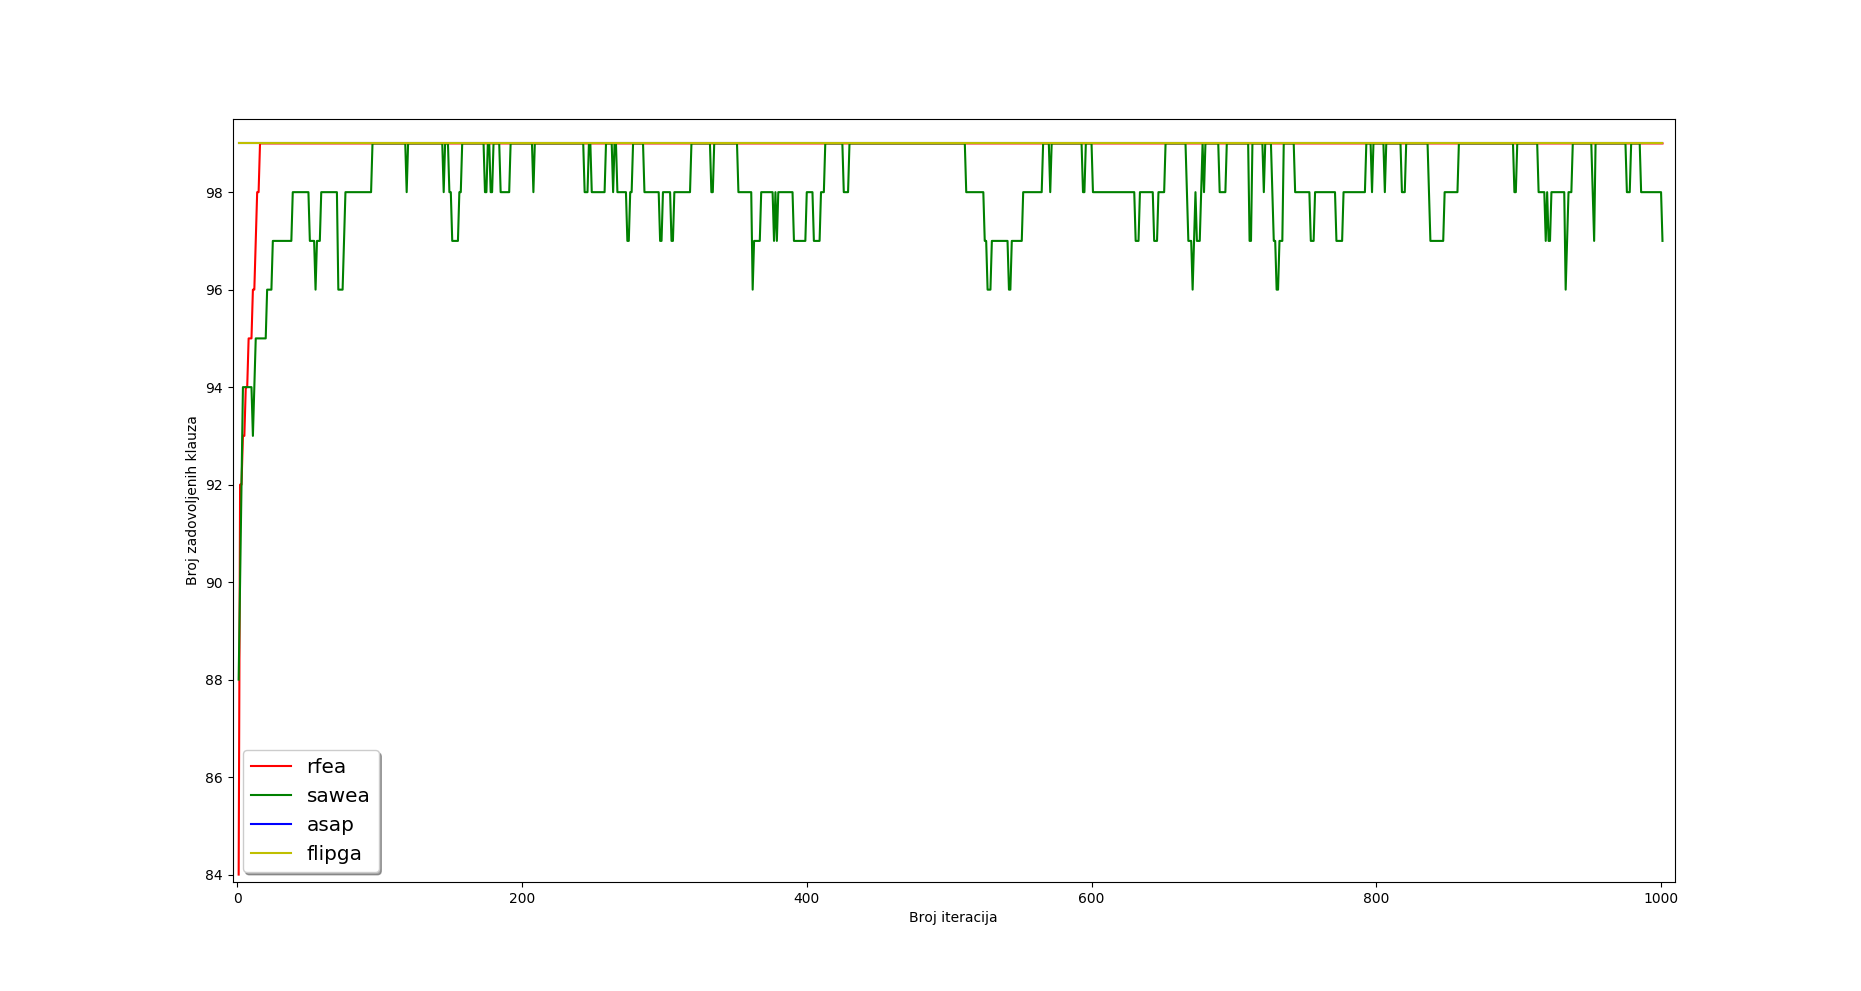
\includegraphics[width=\textwidth]{ea-aim-50-2_0-no}
\caption{Broj zadovoljenih klauza kroz iteracije za aim-50-2\_0-no}\label{img:ea_no1}
\end{figure}

Na slici \ref{img:ea_no2} prikazano je rešavanje nešto teže nezadovoljive instance.
I dalje su za čitavu klasu razlike FlipGA (6,19s) i ASAP (0,59s) pri čemu se još jasnije 
vidi značaj ASAP unapređenja. RFEA (649,24s) pokazao se još gori za teže instance. 
On, istina, monotono raste pri uspehu u pretrazi, za razliku od SAWEA (1,84s) koji više 
nasumično luta, ali kada se pogleda vreme izvršavanja, to definitivno nije vredno.
Takođe, SAWEA u svom lutanju uspeva da dođe do rešenja, za razliku od RFEA
koji je očigledno dostigao svoj lokalni optimum.\\
 
\begin{figure}[h!]
\centering
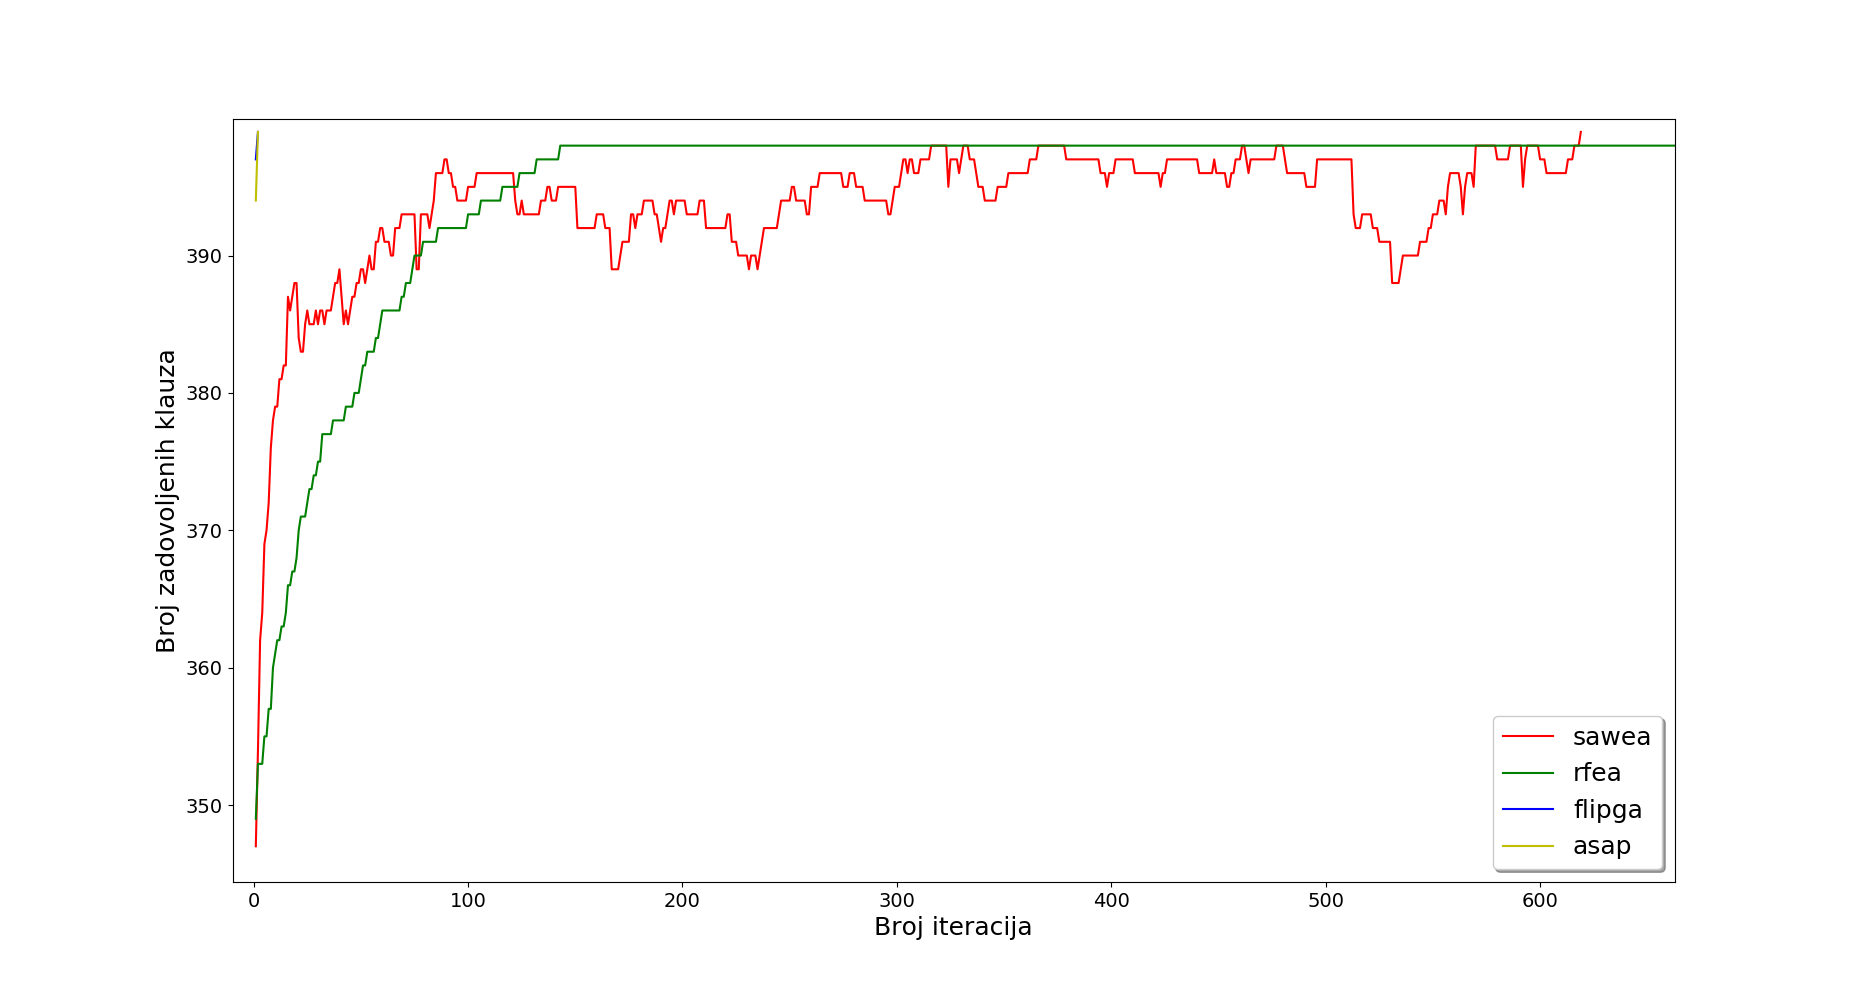
\includegraphics[width=\textwidth]{ea-aim-200-2_0-no}
\caption{aim-200-2\_0-no}\label{img:ea_no2}
\end{figure}

Potom je vršeno poređenje za zadovoljive testove, gde su rezultati u tabeli \ref{tab:ea_SAT}.
Iz rezultata vidi se slična situacija kao i u prethodnoj grupi, samo ovoga puta 
SAWEA i RFEA daleko odstupaju od preostala dva unapređenja lokalnom pretragom.
RFEA se po rezultatima čini nešto bolji, ali kada je vreme izvršavanja u pitanju, to
apsolutno nije opravdano. Slično je i pri poređenju FlipGA i ASAP gde su oba postigli
iste rezultate u svim instancama, pri čemu je ASAP neuporedivo brži.\\

\begin{table}[h!]
\centering
\captionof{table}{AIM zadovoljivi testovi}\label{tab:ea_SAT} 
\begin{tabular}{ |p{2.5cm}|p{1.4cm}|p{1.4cm}||p{1.6cm}|p{1.6cm}|p{1.6cm}|p{1.6cm}|}
\hline
 Instanca & Broj \break literala & Broj \break klauza & SAWEA & RFEA & FlipGA & ASAP \\ 
 \hline
 aim-50-1\_6-yes & 50 & 80 & 79 & 79 & 79 &  79 \\ 
 aim-50-2\_0-yes &  & 100 &  98.4 &  99 & 99 & 99 \\ 
 aim-50-3\_4-yes &  & 170 & 167 & 167.2 & 170 & 170  \\ 
 aim-50-6\_0-yes &  & 300 &  300 & 290 &  300 &  300 \\ 
 \hline
 aim-100-1\_6-yes & 100 & 160 & 158.2 & 158 &  159 & 159 \\ 
 aim-100-2\_0-yes &  & 200 & 195.8 &  197.8 & 199 &  199 \\ 
 aim-100-3\_4-yes &  & 340 & 324.6  & 332.4 & 340 & 340 \\ 
 aim-100-6\_0-yes &  & 600 &  586.8 & 576 & \textbf{600} & 600 \\ 
 \hline
 aim-200-2\_0-yes & 200 & 400 &  392.2 & 396 & 399 & 399 \\ 
 aim-200-6\_0-yes &  & 1200 & 1133 & 1173 &  1200 & 1200 \\ 
 \hline
\end{tabular} 
\end{table}


Jedna instanca zadovoljivih problema prikazana je na slici \ref{img:ea_yes1}.
U skladu sa uočenom monotonošću RFEA (12,27s) koja se dobija zahvaljujući komplikovanijem
izračunavanju funkcije prilagođenosti $f_{REF}$ uspela je da ga istakne pre 
SAWEA (0,86s) po broju iteracija. Ali po brzini
izvršavanja i dalje ostaje najgore rangiran. ASAP (0,11s) i FlipGA (0,61s) 
došli su do rešenja u prvoj iteraciji. \\

\begin{figure}[h!]
\centering
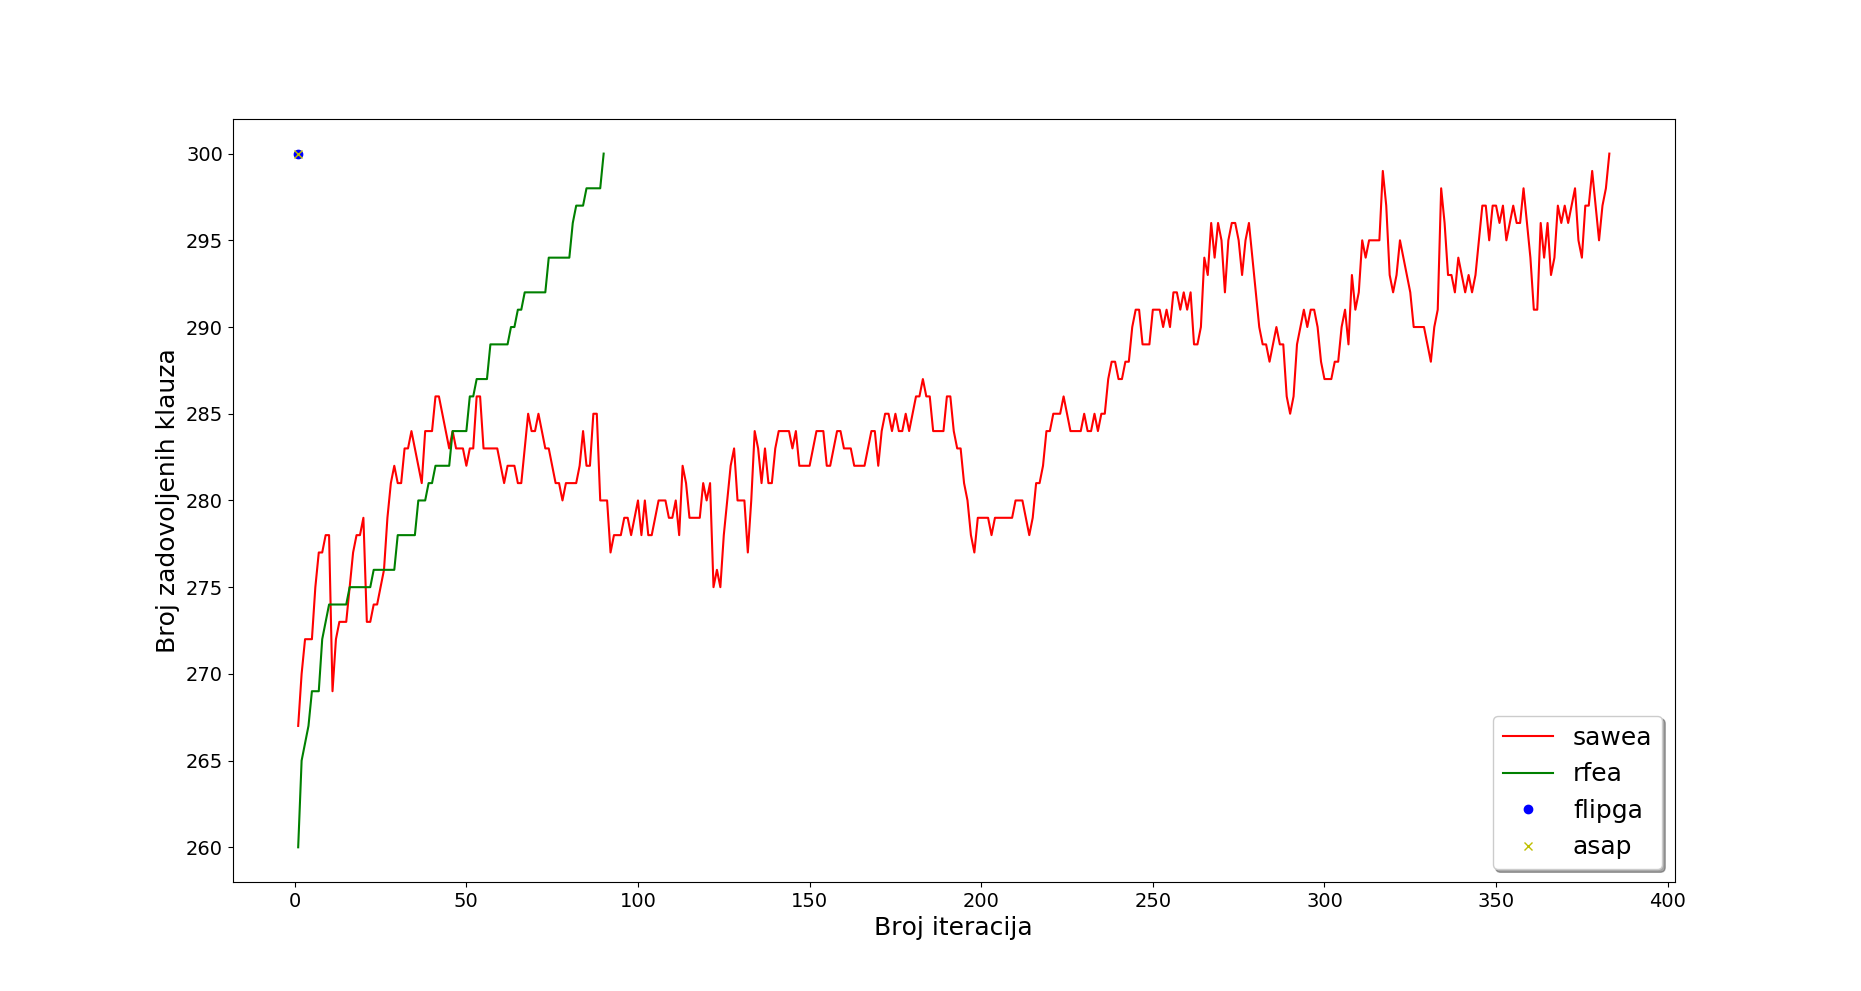
\includegraphics[width=\textwidth]{ea-aim-50-6_0-yes}
\caption{aim-50-6\_0-yes}\label{img:ea_yes1}
\end{figure}


\newpage


\section{Optimizacija rojem čestica (PSO)}
\label{sec:pso}
Optimizacija rojem čestica (Particle swarm optimization – PSO) je jedna od 
tehnika pretraživanja zasnovana na populaciji kao što je genetski algoritam, ali
originalno ne koriste evolutivne procedure kao što su mutacija i ukrštanje.
PSO algoritmi su 1995. godine uveli Kenedi i Eberhart kao 
alternativu standardnim genetskim algoritmima. \\

Optimizacija rojem čestica je algoritam zasnovan na ponašanju pojedinačnih jedinki unutar određene grupe (na primer, jata ptica ili roja insekata). Ukoliko se, vođeno instiktom, jato prica uputi u određenom smeru u potrazi za hranom, očekivanje je da će čitavo jato slediti upravo onu pticu koja je pronašla izvor hrane. Međutim, i svaka ptica ponaosob može biti vođena sopstvenim instiktom i time na trenutak u potrazi za hranom napustiti jato. Tada se verovatno može desiti da, ukoliko pronađe bolji izvor hrane, čitavo jato upravo krene da sledi tu pticu. \\

PSO pripada skupu algoritama koji se zasnivaju na inteligenciji roja (swarm intelligence). Algoritam radi nad skupom jedinki, koji se naziva rojem. Elementi ovog skupa se nazivaju česticama. 
Svaka čestica predstavlja kandidatsko rešenje optimizacionog problema. Čestice se na unapred definisan način kreću po prostoru pretraživanja. Njihovo kretanje se usmerava imajući u vidu njihovu trenutnu poziciju, njihovu do sada najbolju poziciju, kao i do sada najbolju poziciju čitavog roja. Pod najboljom pozicijom čitavog roja se podrazumeva do sada najbolja pozicija, uzimajući u obzir sva njegova rešenja. Proces se ponavlja dok ne bude zadovoljen kriterijum zaustavljanja, a u svakoj iteraciji se ažurira najbolja vrednost rešenja za svaku česticu, kao i za roj u celini. \\

Neka je dat roj sa $\vec{S}$ čestica. Svaka čestica se sastoji od tri elementa:
\begin{list}{•}{}
	\item Pozicija u prostoru za pretragu $\vec{x_i}$
	\item Brzina, vektor $\vec{v_i}$
	\item Sećanje, koje se koristi za skladištenje elitnih čestica globalne pretrage $\vec{P_g}$, kao i najboljih individualnih rešenja $\vec{P_i}$ koja su do sada pronašle zasebne čestice\\
\end{list}

Nije neophodno da se u budućim populacijama nalazi bilo koji elitni pojedinac, iako svaka čestica u populaciji pokušava da bude blizu svog najboljeg rešenja i globalnog najboljeg rešenja. \\ 


Osnovni oblik PSO algoritma dat je sledećim samoažurirajućim jednačinama: \\ 
\begin{equation}\label{eq:v}
\vec{v_{i}}^{t+1} = w \cdot \vec{v_{i}}^{t} + c_1 \cdot \vec{r_1} \times (\vec{P_{i}}^{t} - \vec{x_{i}}^{t}) + c_2\cdot \vec{r_2} \times (\vec{P_{g}}^{t} - \vec{x_{i}}^{t}) 
\end{equation}

\begin{equation}\label{eq:pos}
\vec{x_{i}}^{t+1} = \vec{x_{i}}^{t} + \vec{v_{i}}^{t+1} 
\end{equation}

Jednačina \ref{eq:v} opisuje kako se ažurira brzina $i$-te čestice, a \ref{eq:pos} koja je sledeća pozicija $i$-te čestice, pri čemu je: 

\begin{list}{•}{}
	\item $w$ - faktor inercije
	\item $c_1, c_2$ - faktori učenja: kognitivna i socijalna
	\item $\vec{v_{id}}^{t}$ - brzina $i$-te čestice u iteraciji $t$ 
	\item $\vec{x_{id}}^{t}$ - pozicija $i$-te čestice u iteraciji $t$ 
	\item $\vec{r_1}, \vec{r_2}$ - pseudoslučajni brojevi iz uniformnog intervala $[0,1]$
	\item $\vec{P_i}$ - najbolje individualno rešenje čestice $i$
	\item $\vec{P_g}$ - trenutno najbolje globalno rešenje\\ 
\end{list}

Kako je max k-SAT problem diskretan potrebno je prilagoditi jednačinu \ref{eq:pos}. Izračunata brzina $\vec{v_{i}}$ je iz $\mathbb{R}^n$, pa je potrebno da se svede na $\{ 0,1 \}^n$. Jedan predlog za ažuriranje položaja čestice, izložen u radu \cite{sigmoid}, dat je sigmoidnom transformacijom. Sada ${v_{i}}^{t}$ predstavlja verovatnoću da bit $x_{i}^{t}$ uzme vrednost 1.  \\

\begin{equation}\label{eq:posSIGMOID}
x_{i}^{t}=\begin{cases}
               1, rand(0,1) < sigmoid(v_{i}^{t})\\
               0, inace\\
            \end{cases}
\end{equation}\label{eq:sigmoid}
\begin{equation}
sigmoid(v_{i}^{t}) = \frac{1}{1+e^{-v_{i}^{t}}}
\end{equation}
 
 
\subsection{Pseudokod PSO}
\label{sec:pso_pseudokod}
U ovom poglavlju dat je osnovni oblik algoritma na kojem se zasnivaju ostale varijante i izmene koje će biti detaljnije izložene. Jednu populaciju, odnosno roj, čini unapred određen broj čestica, lista potencijalnih rešenja kao i dodeljene brzine za svaku od njih. 
Kroz iteracije računa se fitnes, aužuriraju se brzine i pozicije čestica dok se ne zadovolji kriterijum zaustavljanja. 
Jedna varijanta (WPSOSAT) uvodi i lokalnu pretragu koja se izvodi umesto ažuriranja pozicija, odnosno jednačine \ref{eq:posSIGMOID}.
Kriterijumi zaustavljanja koji se mogu koristiti u opštem slučaju su: da li je dostignut maksimalan broj unapred zadatih iteracija ili, da li u poslednjih nekoliko iteracija nema značajnog napretka.
U test primerima za koje unapred znamo da je formula zadovoljiva, ili koliko je klauza zadovoljivo, možemo koristiti kriterijum da se dostigao ukupan broj zadovoljivih klauza. \\

\begin{algorithm}[H]
\SetAlgoLined
\SetKwInOut{Input}{Input}
\SetKwInOut{Output}{Output}

\Input{Formula $F$ u KNF-u, $n$ i $m$}
\Output{Najbolja procenjena valuacija i broj zadovoljenih klauza}
\BlankLine
 inicijalizacija populacije: pozicije i brzine\;
 t = 0; \tcp*[h]{tekuća iteracija}\\
 \While{nije zadovoljen uslov zaustavljanja}{
  t = t + 1\;
  \For{$i\leftarrow 0$ \KwTo broj cestica u roju}{
  	Izračunaj $Fitness$($\vec{P_i^t}$)\;
  	Sačuvaj individualni najbolji rezultat kao globalni $\vec{P_g}$\;
  	Ažuriraj brzine na osnovu $\vec{P_i}$ i $\vec{P_g}$\;
  	Ažuriraj pozicije $\vec{v_i^t}$\;
  	Ažuriraj individualni najbolji rezultat $\vec{P_i}$\;
  	Ažuriraj globalni najbolji rezultat $\vec{P_g}$\;
  }
 }
\caption{Osnovni PSO algoritam}
\end{algorithm}


\subsection{Inicijalizacija rešenja}
\label{sec:pso_init}
Potrebno je inicijalizovati pozicije čestica i vektora brzine. Pozicije su inicijalizovane pseudo-slučajnim brojevima $\{0,1\}$, a vektor brzine realnim brojevima iz intervala $[-V_{min}, V_{max}]$, gde su granice intervala jedan od parametara PSO algoritma.


\subsection{Fitnes funkcija}
\label{sec:pso_fitness}
Fitnes funkcija je veoma važna za perfomanse algoritma.
Prva fitnes funkcija koja se sama nameće jeste broj zadovoljenih klauza, kakva je data u samoj formulaciji problema, ali se takva funkcija nije pokazala kao dovoljno dobra. Bolji mehanizam je stepenasto ažuriranje težina (SAW - stepwise adaptation weights) uvedena od strane Eiben-a \cite{fitnes}. Ona je data sledećim formulama:

\begin{equation}\label{eq:SAW}
F_{SAW}(x) = \sum_{i=1}^{m} W_iC_i(x)
\end{equation}

\begin{equation}\label{eq:wForSAW}
W_{i+1} = W_{i} + 1 - C_i(x^*)
\end{equation}

Svakoj klauzi $C_i$ dodeljuje se težina $W_i$. Ova funkcija ima za cilj identifikovanje težih klauza u procesu učenja koja je predstavljena većom vrednošću $W_i$. Na početku su težine inicijalizovane na 1, pa se potom ažuriraju jednačinom \ref{eq:wForSAW}. $x^*$ je tekuće najbolje rešenje.


\subsection{Varijante PSO algoritma}
\label{sec:pso_varijante}

Da bismo uporedili kombinaciju lokalne pretrage, SAW fitnes funkcije i klasičnog PSO algoritma implementirani su i testirane sledeće tri verzije: \\

%TODO DAVID
\subsubsection{PSO-LS}
\label{sec:psols}
PSO-LS je osnovna varijanta algoritma koji ne koristi lokalnu pretragu, već sigmoidnu transformaciju, jednačine \ref{eq:v} i \ref{eq:posSIGMOID} za ažuriranje brzina i pozicije čestica. Fitnes funkcija je $F_{SAW}$, sa korišćenjem težina nad klauzama. Karakteriše ga sporija konvergencija do globalnog optimuma, ali pojedinačne iteracije se izvršavaju brže.

\subsubsection{PSOSAT}
\label{sec:psosat}
PSOSAT koristi lokalnu pretragu, ali ne i $F_{SAW}$, pa je funkcija cilja broj zadovoljenih klauza. Mana ovog algoritma je teško izlaženje iz lokalnih optimuma zbog korišćenja fitnes funkcije koja ne razaznaje težinu klauza.

\subsubsection{WPSOSAT}
\label{sec:wpsosat}
WPSOSAT - Modifikovan PSO algoritam sa korišćenjem flip heuristike i $F_{SAW}$ fitnes funkcije. Značaj lokalne pretrage ogleda se u poređenju sa PSO-LS, a korišćenje $F_{SAW}$ u poređenju sa PSOSAT.



\subsection{Rezultati}
\label{sec:pso_rezultati}
%TODO DAVID
Svi algoritmi pokretani su pet puta sa istim parametrima i beležen je prosečan broj zadovoljenih klauza, pri čemu podebljan rezultat označava da se do rešenja dolazilo u prvoj iteraciji. U tabeli \ref{tab:UNSAT} skoro svi algoritmi su uspeli da brzo nađu rešenje. Za sada između PSOSAT i WPSOSAT nema razlike. Već za poslednji test vidi se slabost ne korišćenja lokalne pretrage. Već u tabeli \ref{tab:SAT} PSO-LS nije mogao da se uporedi sa ostala dva algoritma. Za neke instance do globalnog optimuma došao je jedino WPSOSAT odakle se vidi značaj SAW funkcije.

\begin{table}[h!]
\centering
\captionof{table}{Parametri}\label{tab:parametri} 
\begin{tabular}{ |p{3cm}|p{2cm}| }
 \hline
 Parametar 	& Vrednost \\ 
 \hline
 Broj iteracija & 1000 \\
 w & 1 \\
 c1 & 1.7 \\
 c2 & 2.1 \\
 Broj čestica	& 20 \\
 max flip & 30000 \\
 $v_{min}$ & -1 \\
 $v_{max}$ & 1\\ 
 \hline
\end{tabular}
\end{table}


\begin{table}[h!]
\centering
\captionof{table}{AIM nezadovoljivi testovi}\label{tab:UNSAT}
\begin{tabular}{ |p{2.5cm}|p{1.4cm}|p{1.4cm}||p{1.6cm}|p{1.6cm}|p{1.6cm}| } 
\hline
 Instanca & Broj \break literala & Broj \break klauza & PSO-LS & PSOSAT & WPSOSAT \\ 
 \hline
 aim-50-1\_6-no & 50 & 80 & 79 & \textbf{79} & \textbf{79} \\ 
 aim-50-2\_0-no & 50 & 100 & 99 & \textbf{99} & \textbf{99} \\
 aim-100-1\_6-no & 100 & 160 & 159 & \textbf{159} & \textbf{159} \\
 aim-100-2\_0-no & 100 & 200 & 199 & \textbf{199} & \textbf{199} \\
 aim-200-2\_0-no & 200 & 400 & 398.6 & \textbf{399} & \textbf{399} \\
 \hline
\end{tabular}
\end{table}

\begin{table}[h!]
\centering
\captionof{table}{AIM zadovoljivi testovi}\label{tab:SAT} 
\begin{tabular}{ |p{2.5cm}|p{1.4cm}|p{1.4cm}||p{1.6cm}|p{1.6cm}|p{1.6cm}|}
\hline
 Instanca & Broj \break literala & Broj \break klauza & PSO-LS & PSOSAT & WPSOSAT \\
 \hline
 aim-50-1\_6-yes & 50 & 80 & 79 & 79.2 & 80 \\
 aim-50-2\_0-yes &  & 100 & 99 & 99 & 100 \\
 aim-50-3\_4-yes &  & 170 & 168.6 & 170 & 170 \\
 aim-50-6\_0-yes &  & 300 & 300 & 300 & 300 \\
 \hline
 aim-100-1\_6-yes & 100 & 160 & 158.6 & 159 & 159 \\
 aim-100-2\_0-yes &  & 200 & 198 & 199 & 200 \\
 aim-100-3\_4-yes &  & 340 & 328 & 339.4 & 340 \\ 
 aim-100-6\_0-yes &  & 600 & 580.2 & \textbf{600} & \textbf{600} \\
 \hline
 aim-200-2\_0-yes & 200 & 400 & 395.4 & 399 & 399 \\
 aim-200-6\_0-yes &  & 1200 & 1135.6 & \textbf{1200} & \textbf{1200} \\ 
 \hline
\end{tabular}
\end{table}

%TODO Poredjenje sa rezultatima EA

\section{Zaključak}
\label{sec:zakljucak}
%TODO

\addcontentsline{toc}{section}{Literatura}
\appendix
\bibliography{max-k-sat} 
\bibliographystyle{plain}

\end{document}
